\documentclass[landscape,a0paper,fontscale=0.292]{baposter}

\usepackage[vlined]{algorithm2e}
\usepackage{times}
\usepackage{calc}
\usepackage{url}
\usepackage{graphicx}
\usepackage{amsmath}
\usepackage{amssymb}
\usepackage{relsize}
\usepackage{multirow}
\usepackage{booktabs}

\usepackage{graphicx}
\usepackage{multicol}
\usepackage[T1]{fontenc}
\usepackage{ae}
\usepackage{enumitem}

\usepackage{colortbl}
\usepackage{xcolor}
%\usepackage{gensymb} % for \degree
\graphicspath{{images/}}

\setlist[itemize]{leftmargin=*,nosep}
    \setlength{\columnsep}{0.7em}
    \setlength{\columnseprule}{0mm}

\setlist[enumerate]{leftmargin=2.5em,nosep}
    \setlength{\columnsep}{1.0em}
    \setlength{\columnseprule}{0mm}

% %%%%%%%%%%%%%%%%%%%%%%%%%%%%%%%%%%%%%%%%%%%%%%%%%%%%%%%%%%%%%%%%%%%%%%%%%%%%%%%%
% % Save space in lists. Use this after the opening of the list
% %%%%%%%%%%%%%%%%%%%%%%%%%%%%%%%%%%%%%%%%%%%%%%%%%%%%%%%%%%%%%%%%%%%%%%%%%%%%%%%%
% \newcommand{\compresslist}{%
% \setlength{\itemsep}{0pt}%
% \setlength{\itemsep}{0pt}%
% \setlength{\parskip}{0pt}%
% \setlength{\parsep}{0pt}%
% }
\renewcommand{\rmdefault}{ptm} % Arial
\renewcommand{\sfdefault}{ptm} % Arial

\newcommand{\vn}{\boldsymbol{n}}
\newcommand{\vl}{\boldsymbol{l}}
\newcommand{\vM}{\mathbf{M}}
\newcommand{\vN}{\mathbf{N}}
\newcommand{\vL}{\mathbf{L}}
%%%%%%%%%%%%%%%%%%%%%%%%%%%%%%%%%%%%%%%%%%%%%%%%%%%%%%%%%%%%%%%%%%%%%%%%%%%%%
%% Begin of Document
%%%%%%%%%%%%%%%%%%%%%%%%%%%%%%%%%%%%%%%%%%%%%%%%%%%%%%%%%%%%%%%%%%%%%%%%%%%%%
\begin{document}
%%%%%%%%%%%%%%%%%%%%%%%%%%%%%%%%%%%%%%%%%%%%%%%%%%%%%%%%%%%%%%%%%%%%%%%%%%%%%
%% Here starts the poster
%%---------------------------------------------------------------------------
%% Format it to your taste with the options
%%%%%%%%%%%%%%%%%%%%%%%%%%%%%%%%%%%%%%%%%%%%%%%%%%%%%%%%%%%%%%%%%%%%%%%%%%%%%
\begin{poster}{
    % Show grid to help with alignment
    grid=false,
    columns=5,
    % Column spacing
    colspacing=0.7em,
    % Color style
    headerColorOne=cyan!20!white!90!black,
    borderColor=cyan!30!white!90!black,
    % Format of textbox
    textborder=faded,
    % Format of text header
    headerborder=open,
    headershape=roundedright,
    headershade=plain,
    background=none,
    bgColorOne=cyan!10!white,
    headerheight=0.12\textheight
}
% Eye Catcher
{
    
\includegraphics[width=0.045\linewidth]{logo/HKU_logo}
    \makebox[0.005\textwidth]{} 
    \raisebox{0.07\height}{
\includegraphics[width=0.045\linewidth]{logo/oxford_logo}}
    \makebox[0.005\textwidth]{} 
    \raisebox{0.07\height}{
\includegraphics[width=0.045\linewidth]{logo/pku_logo}}
    \makebox[0.005\textwidth]{} 
    \raisebox{0.07\height}{
\includegraphics[width=0.045\linewidth]{logo/pclab_logo}}
    \makebox[0.005\textwidth]{} 
    \raisebox{0.07\height}{
\includegraphics[width=0.045\linewidth]{logo/osaka_logo}}
}
% Title
{
    \sc\huge\bf Self-calibrating Deep Photometric Stereo Networks
}
% Authors
{
    \vspace{0.3em} Guanying Chen$^1$ \enspace Kai Han$^2$ \enspace Boxin Shi$^{3,4}$ \enspace Yasuyuki Matsushita$^5$ \enspace Kwan-Yee K. Wong$^1$ \\[0.2em]
    {$^1$The University of Hong Kong \enspace$^2$University of Oxford \\[0.1em] $^3$Peking University \enspace$^4$Peng Cheng Laboratory \enspace$^5$Osaka University}
}
% University logo
{
    \begin{tabular}{c}
        \raisebox{-1.0\height}{
\includegraphics[width=0.15\linewidth]{CVPRLogo}}\\
        \raisebox{-0.7\height}{
\includegraphics[width=0.16\linewidth]{images/QRCode_Link.pdf}}
    \end{tabular}
}

%%%%%%%%%%%%%%%%%%%%%%%%%%%%%%%%%%%%%%%%%%%%%%%%%%%%%%%%%%%%%%%%%%%%%%%%%%%%%%
%%% Now define the boxes that make up the poster
%%%---------------------------------------------------------------------------
%%% Each box has a name and can be placed absolutely or relatively.
%%% The only inconvenience is that you can only specify a relative position 
%%% towards an already declared box. So if you have a box attached to the 
%%% bottom, one to the top and a third one which should be inbetween, you 
%%% have to specify the top and bottom boxes before you specify the middle 
%%% box.
%%%%%%%%%%%%%%%%%%%%%%%%%%%%%%%%%%%%%%%%%%%%%%%%%%%%%%%%%%%%%%%%%%%%%%%%%%%%%%

%%%%%%%%%%%%%%%%%%%%%%%%%%%%%%%%%%%%%%%%%%%%%%%%%%%%%%%%%%%%%%%%%%%%%%%%%%%%%%
\headerbox{\bf\color{blue} Problem Definition and Contribution}{name=contribution,column=0,row=0,span=2}{
    \textbf{\color{blue}Goal:} Estimating the normal map of a non-Lambertian surface with unknown isotropic reflectances observed under unknown varying light directions. 

    \textbf{\color{blue}Motivations:}
    \begin{itemize}
        \item Traditional methods for uncalibrated photometric stereo often assume a simplified reflectance model.
        \item Recent learning based methods for photometric stereo often assume known light directions. 
        \item The performance of the existing learning based method for uncalibrated photometric stereo~(\textit{i.e.}, the single-stage method UPS-FCN~[1]) lags far behind the calibrated methods.
    \end{itemize}  
}

\headerbox{\bf\color{blue} Problem Formulation}{name=formulation,column=0,below=contribution,span=2}{
    %\textbf{\color{blue}Assumption:} Orthographic camera with linear radiometric response and directional lighting.
    \textbf{\color{blue}Image Formation Model:} Consider a non-Lambertian surface whose appearance is described by a general isotropic BRDF $\rho$. Given a surface point with normal $\vn \in \mathbb{R}^3$ being illuminated by the $j$-th incoming lighting with direction $\vl_j \in \mathbb{R}^3$ and intensity $e_j \in \mathbb{R}$, the image formation model can be expressed as
    \vspace{-0.5em}
    \begin{equation*}
        m_j = e_j \rho (\vn, \vl_j)~\text{max}(\vn^\top \vl_j, 0) + \epsilon_j,
    \vspace{-0.5em}
    \end{equation*}
where $m$ represents the measured intensity, $\text{max}(:, 0)$ accounts for attached shadows, and $\epsilon$ accounts for the global illumination effects and noise.

    \textbf{\color{blue}Main Idea:}  We first estimate lightings from the measured intensities, and then solve for the surface normals using the estimated lightings and measured intensities.
}

\headerbox{\bf\color{blue} Method}{name=abstract,column=0,below=formulation,span=2}{
    \textbf{\color{blue}Network Architecture:} 
    \vspace{-0.5em}
    \begin{center}
        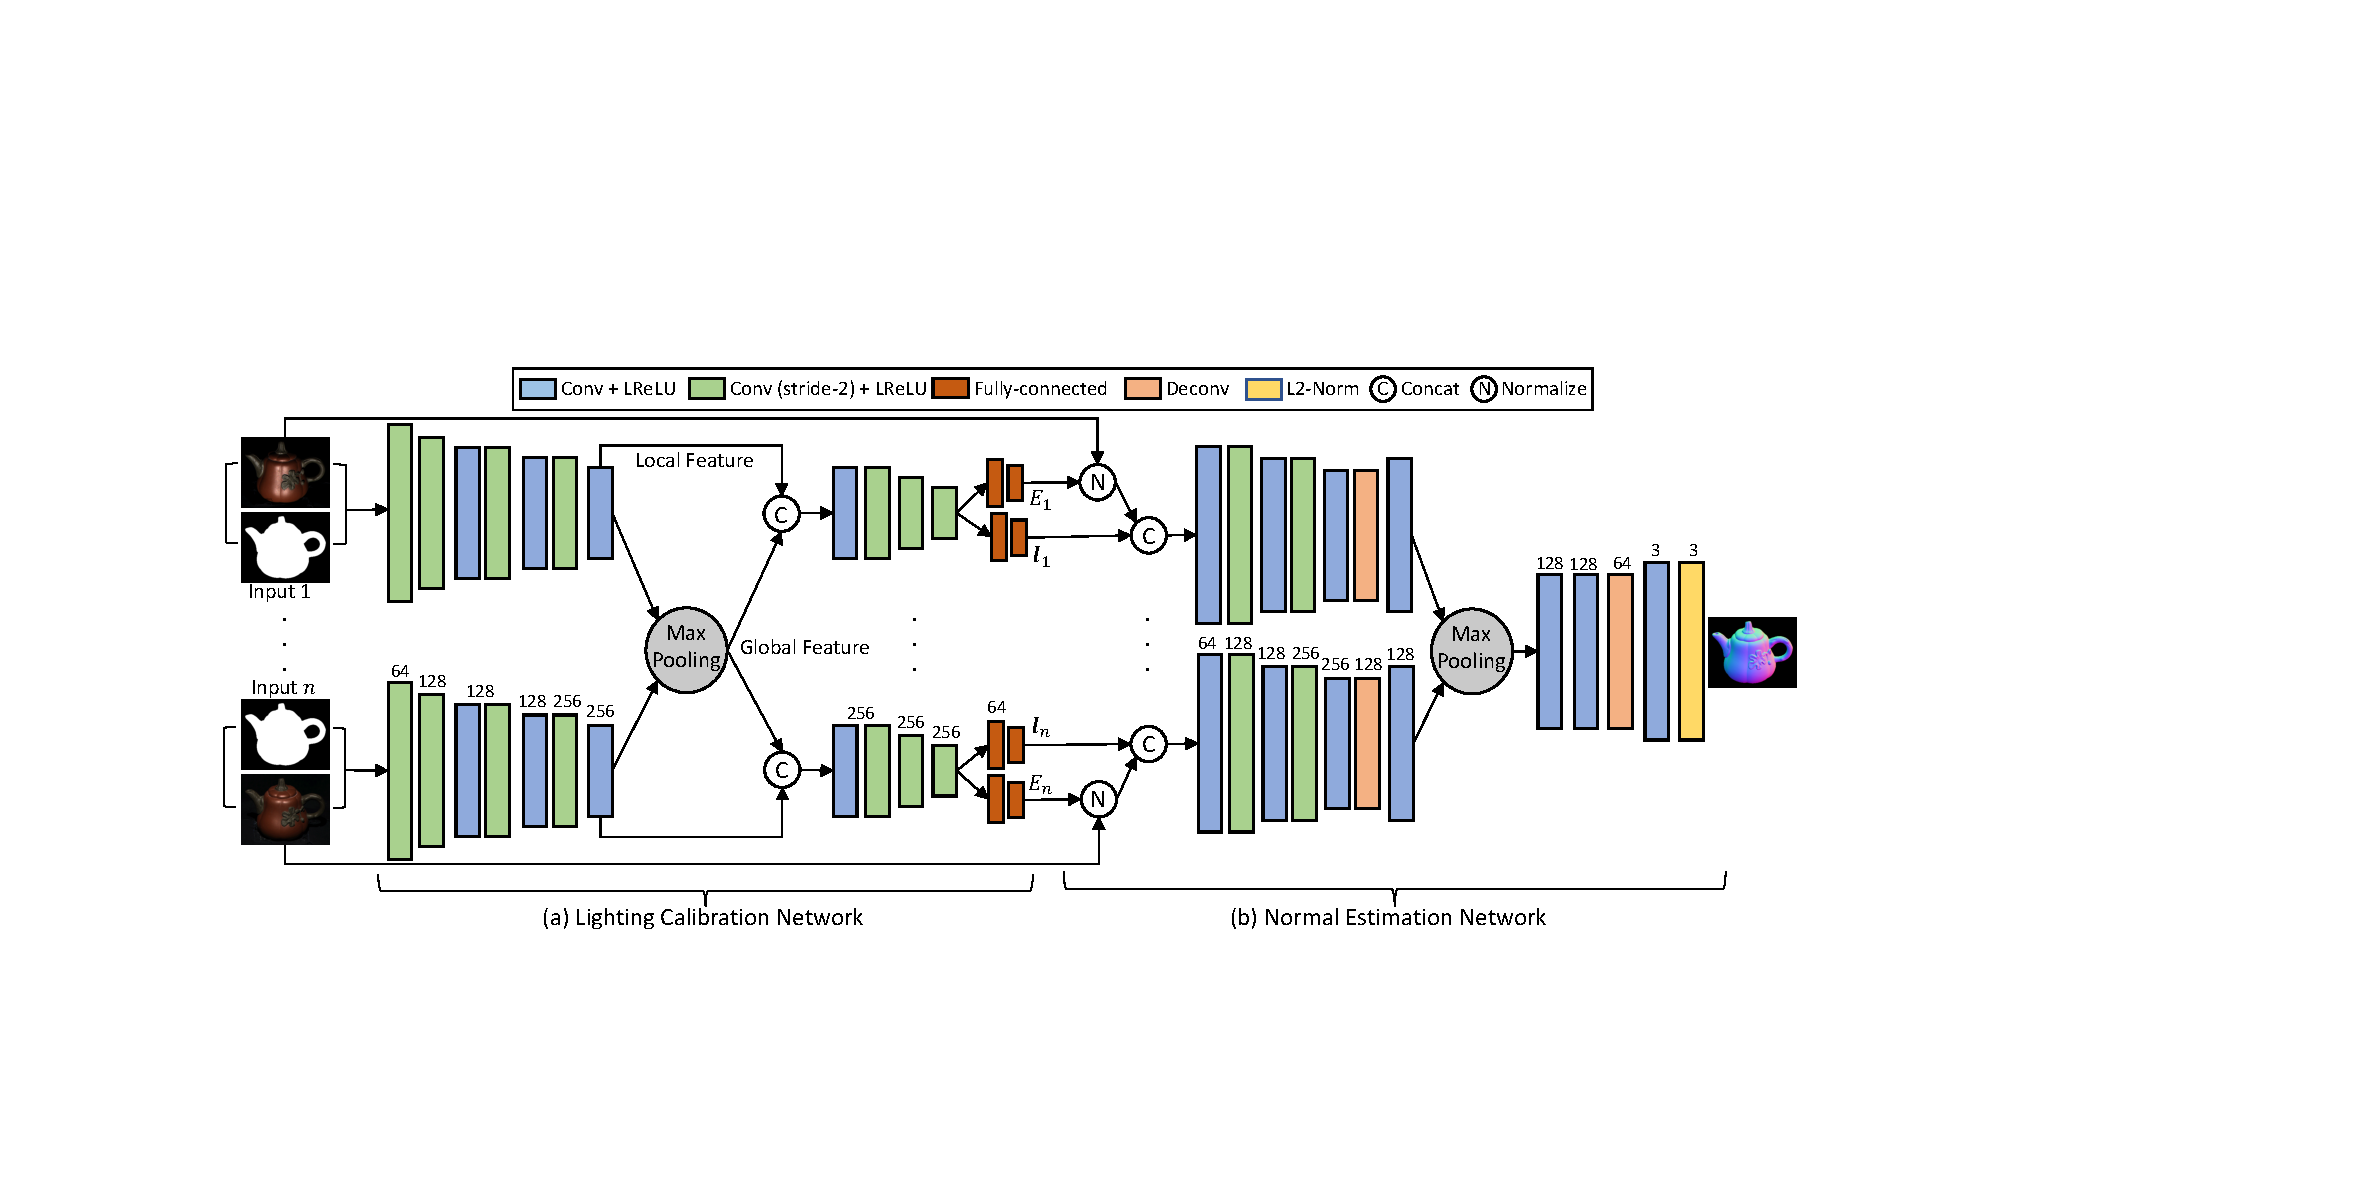
\includegraphics[width=\textwidth]{images/LCNet_NENet.pdf}
    \end{center}

    \begin{minipage}[t]{0.48\linewidth}
        \textbf{\color{blue}Discretization of Lighting Space:}
        \vspace{-0.2em}
        \begin{center}
            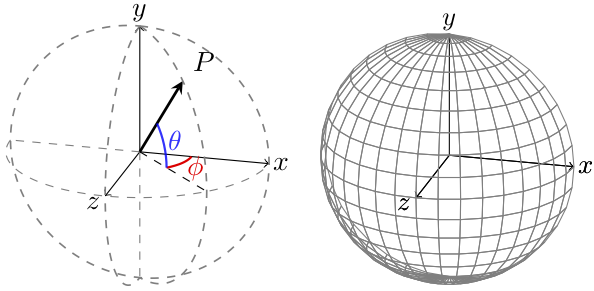
\includegraphics[width=\textwidth]{images/lighting_discretization.png}
        \end{center}
        \vspace{-0.7em}
        \begin{itemize}
            \item Illustration of the coordinate system (left)
            \item Example discretization (right)
        \end{itemize}
    \end{minipage}
    \hfill
    \begin{minipage}[t]{0.48\linewidth}
        \textbf{\color{blue}Loss Function for Lighting Estimation:}
        \vspace{-0.6em}
        \begin{equation*}
            \mathcal{L}_{\text{Light}} = \lambda_{l_a} \mathcal{L}_{l_a} + \lambda_{l_e} \mathcal{L}_{l_e} + \lambda_e \mathcal{L}_e
            \vspace{-0.6em}
        \end{equation*}
        \begin{itemize}
            \item $\mathcal{L}_{l_a}$: azimuth classification loss
            \item $\mathcal{L}_{l_e}$: elevation classification loss
            \item $\mathcal{L}_e$: light intensity classification loss
        \end{itemize}

        \vspace{0.5em} 
        \textbf{\color{blue}Loss function for Normal Estimation:}
        \vspace{-0.6em}
        \begin{align*}
            \mathcal{L}_{\text{Normal}} = \frac{1}{hw} \sum_{i}^{hw} \left(1 - \vn_i^\top \tilde{\vn}_{i} \right)
        \end{align*}
        \begin{itemize}
            \vspace{-0.6em}
            \item Cosine similarity loss
        \end{itemize}
    \end{minipage}
}
%
\headerbox{\bf\color{blue} Experiments \& Results}{name=results,column=2,row=0,span=3}{
    \begin{minipage}[t]{0.50\textwidth}
        \textbf{\color{blue}Synthetic Training Datasets:} 
        \vspace{-0.8em}
        \begin{center}
            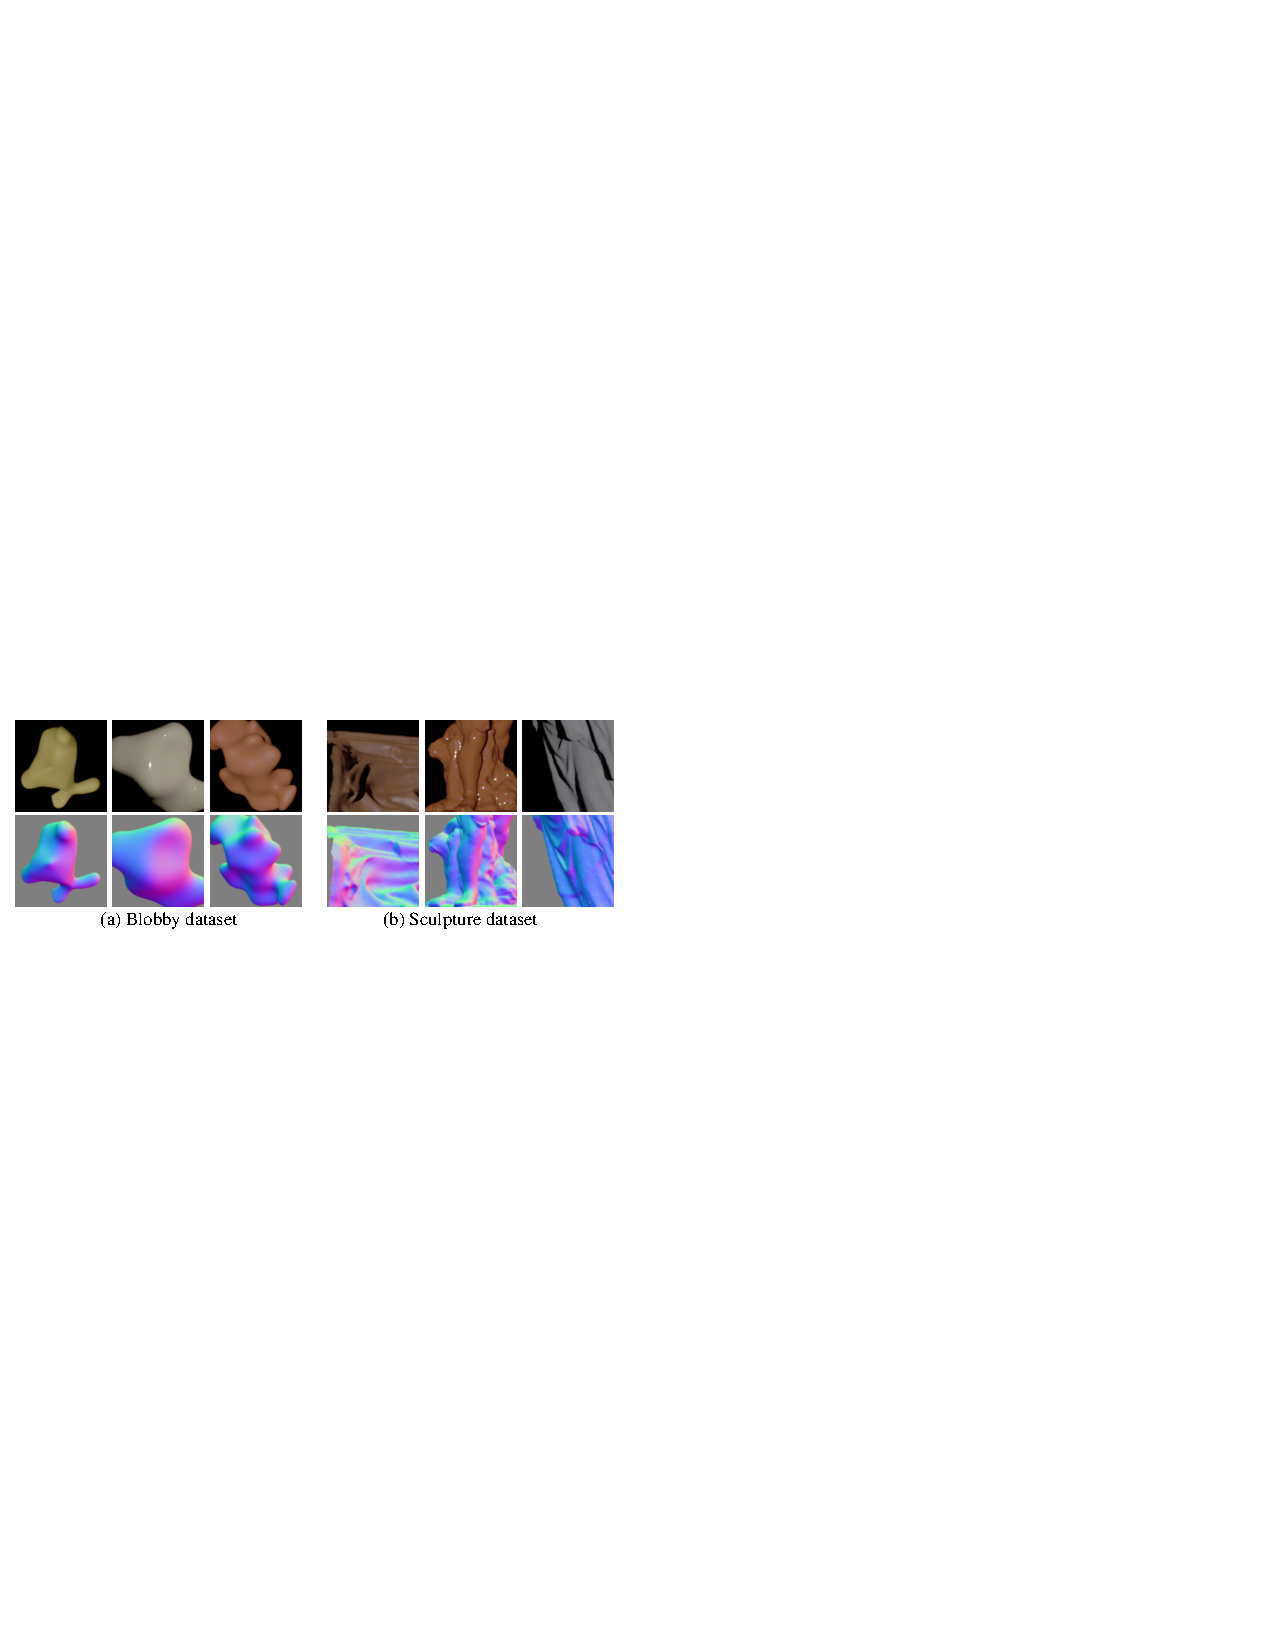
\includegraphics[width=\textwidth]{images/syn_samples.pdf}
        \end{center}

        \vspace{0.1em}
        \textbf{\color{blue}Lighting Distribution of Real Datasets:} 
        \vspace{-0.2em}
        \begin{center}
            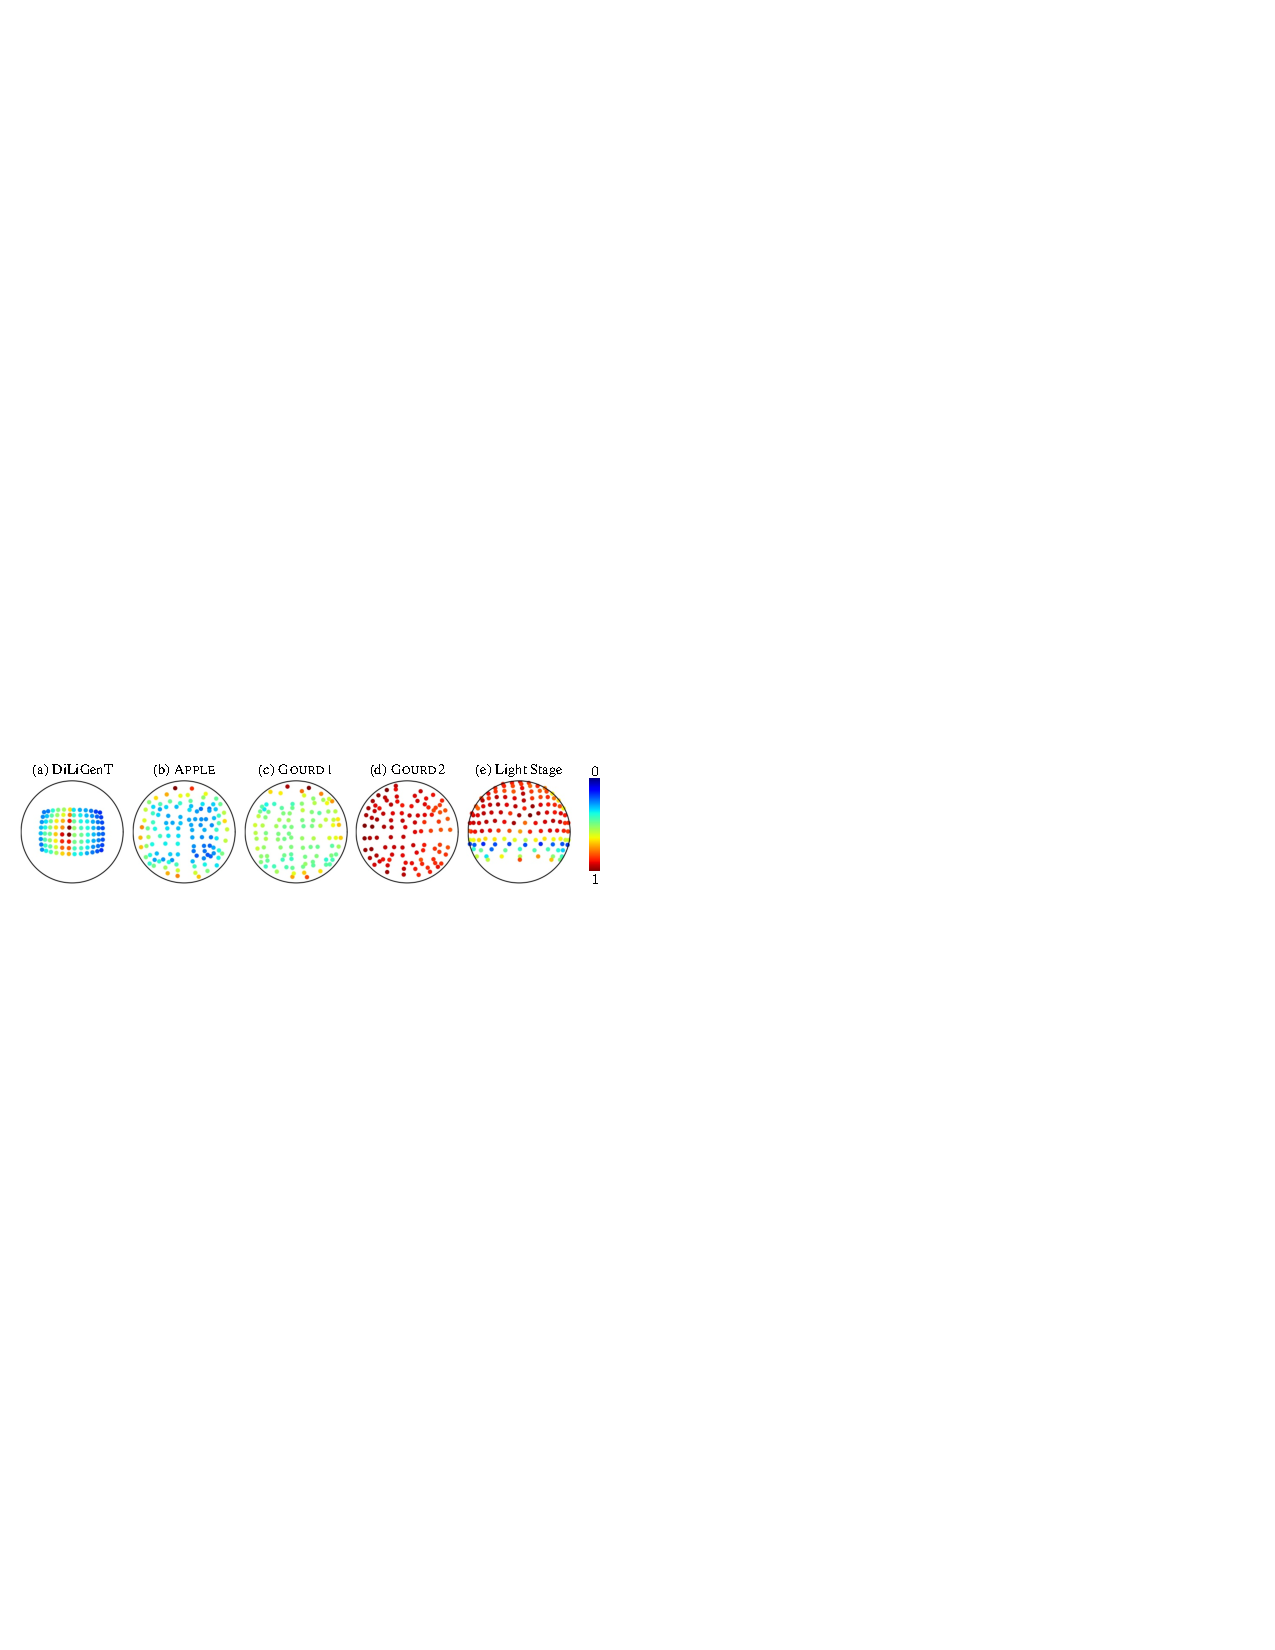
\includegraphics[width=0.95\textwidth]{images/real_lighting_dist.pdf}
        \end{center}
    \end{minipage}\hfill
    \begin{minipage}[t]{0.47\textwidth}
        \textbf{\color{blue}Results on DiLiGenT Benchmark~[2]:} 
        \vspace{-0.2em}
        \begin{center}
            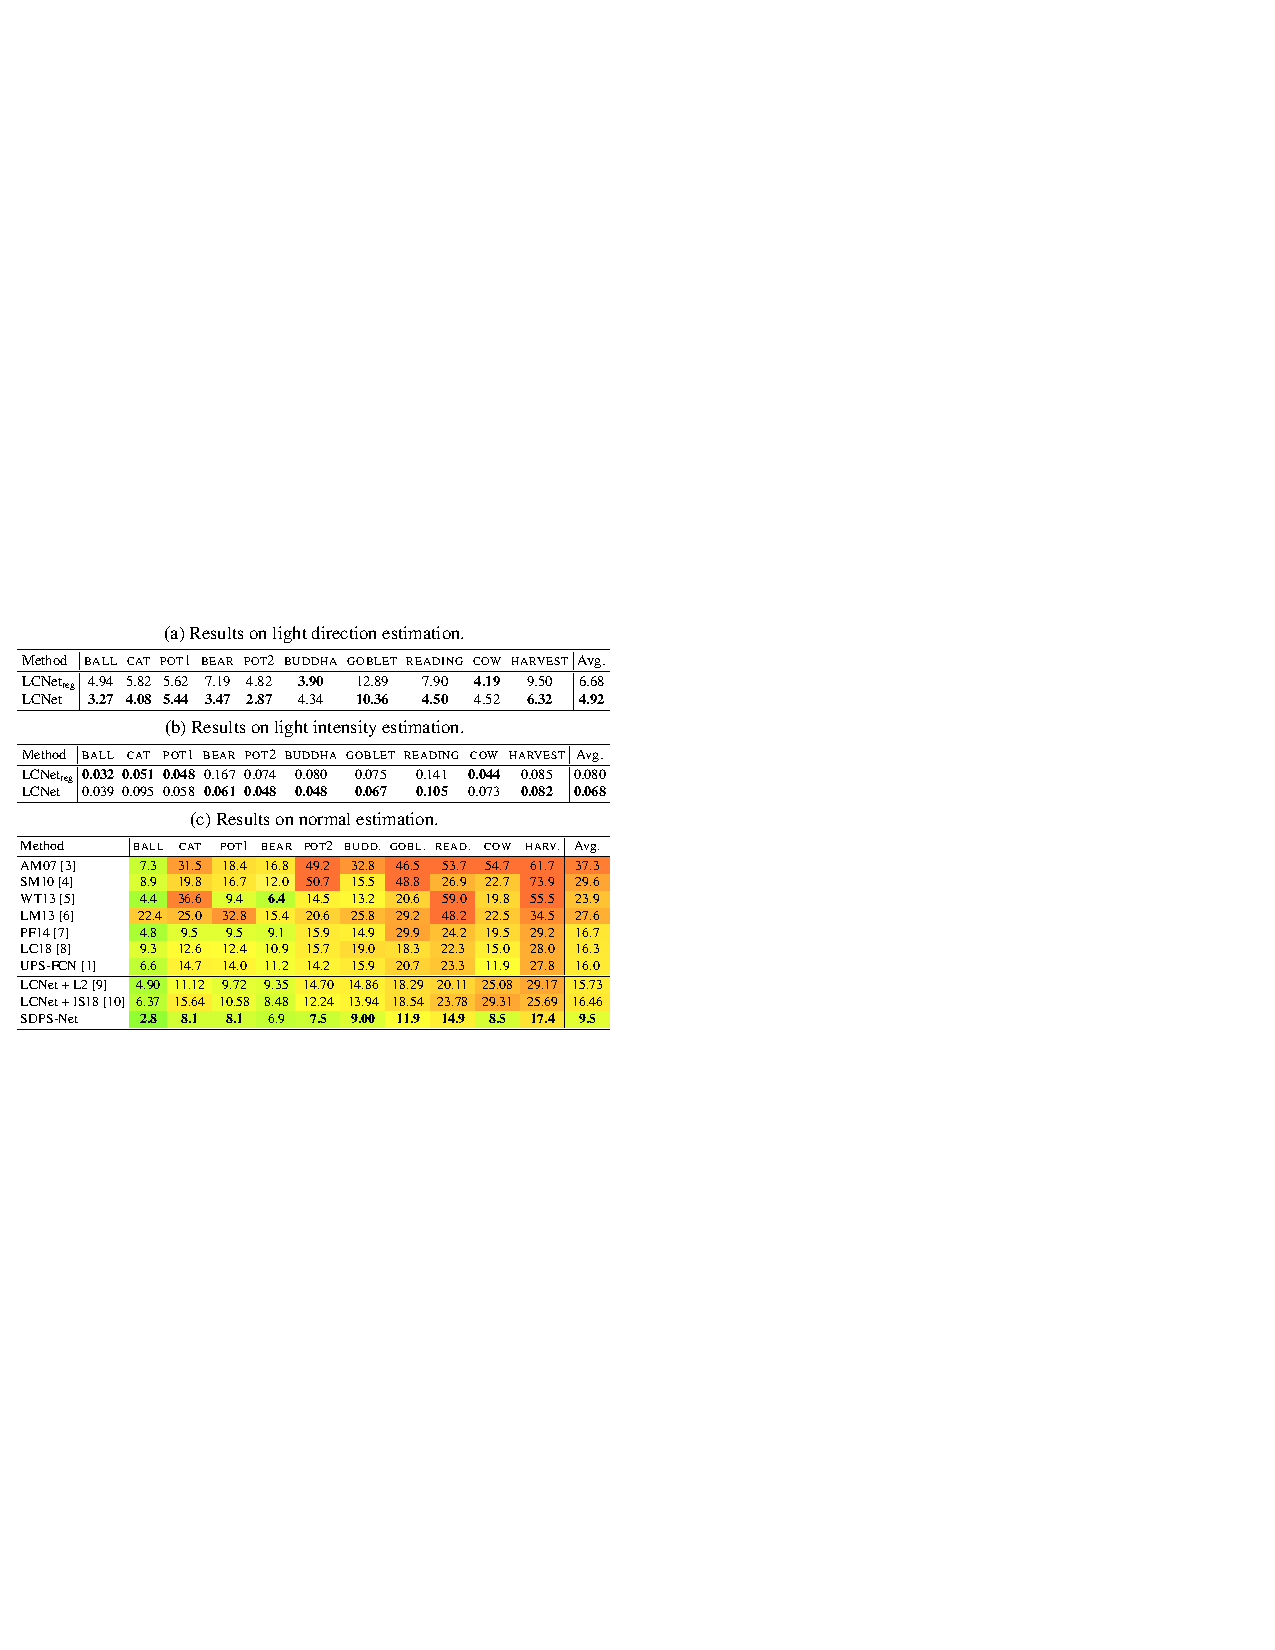
\includegraphics[width=0.98\textwidth]{images/quant_diligent.pdf}
        \end{center}
    \end{minipage}

    \vspace{0.7em}
    \textbf{\color{blue}Quantitative Results on {\sc Bunny} Rendered with $100$ MERL BRDFs:} \\
    \vspace{-1.0em}
    \begin{minipage}[t]{0.23\textwidth}
        \vspace{-9.5em}
        \begin{center}
            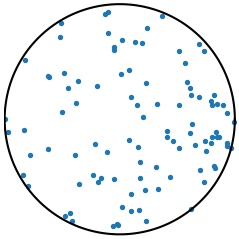
\includegraphics[width=0.48\textwidth]{images/MERL_directions.jpg}
            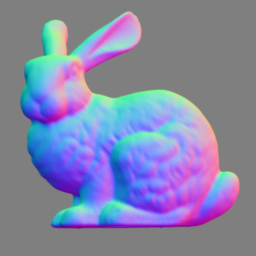
\includegraphics[width=0.48\textwidth]{images/bunny_normal.png}\\
            \vspace{-0.5em}
            \makebox[0.48\textwidth]{\scriptsize (a) Light source} 
            \makebox[0.48\textwidth]{\scriptsize (b) {\sc Bunny}} 
        \end{center}
    \end{minipage}
    \begin{minipage}[t]{0.76\textwidth}
        \begin{center}
            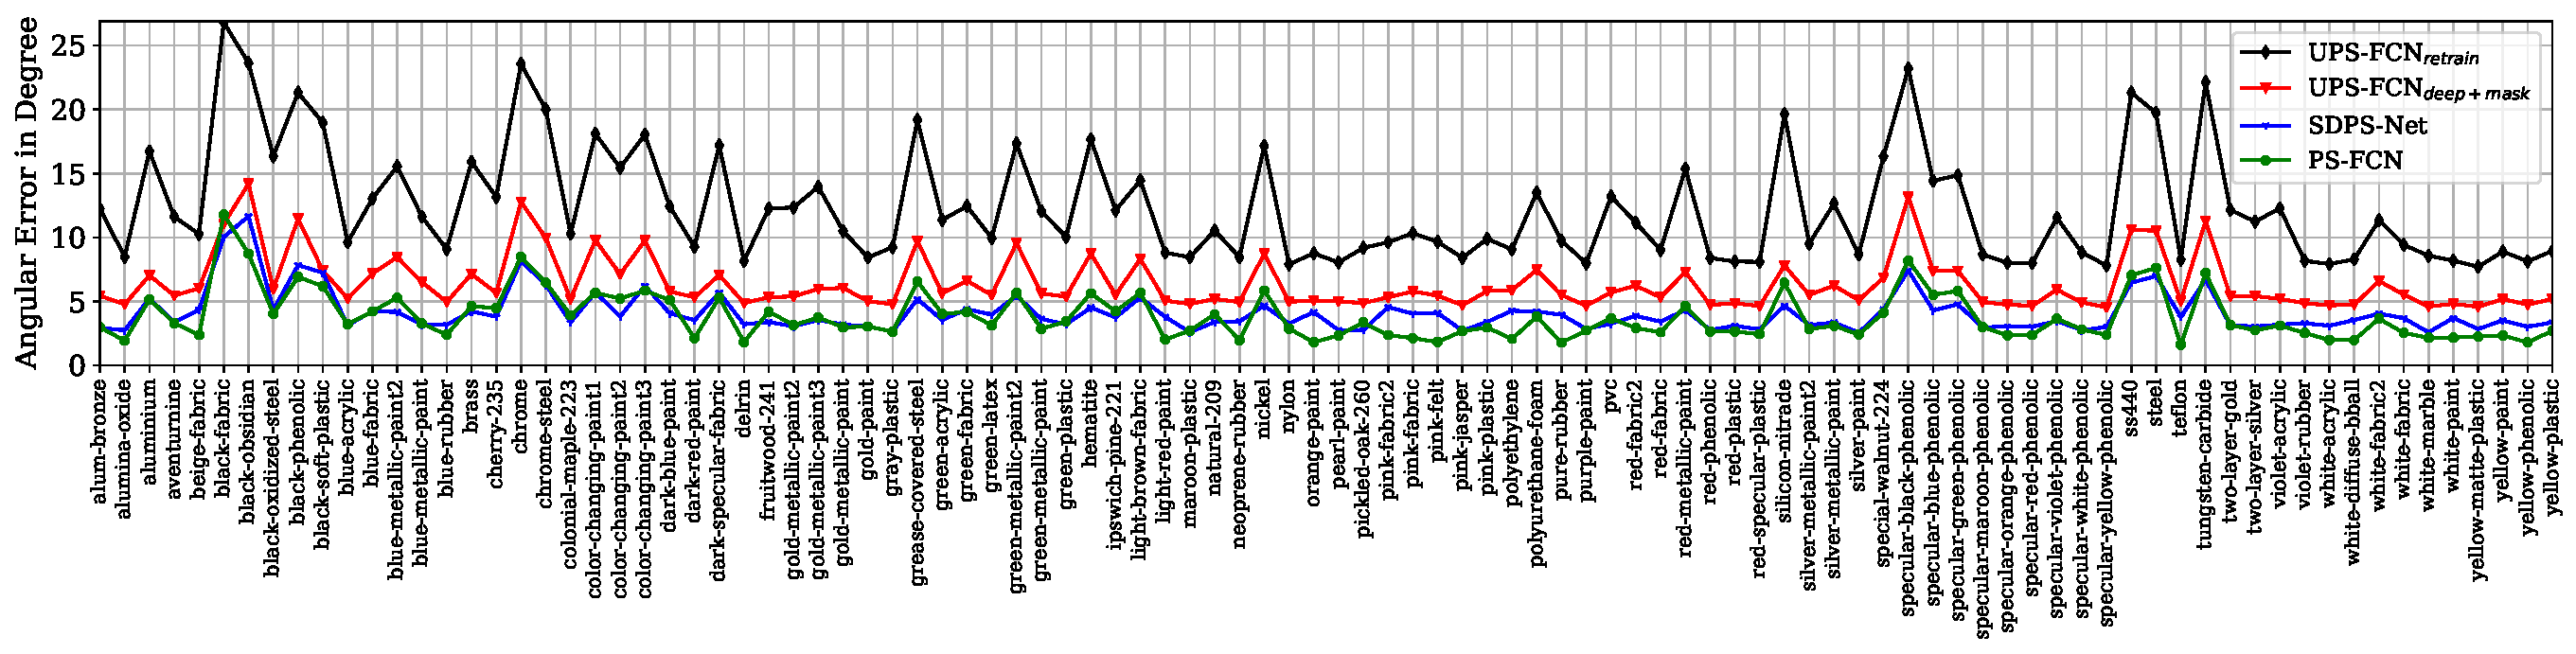
\includegraphics[width=\textwidth]{images/Bunny_100MERL.pdf}
        \end{center}
    \end{minipage}

    \textbf{\color{blue}Quantitaive Comparison on {\sc Harvest} in DiLiGenT Benchmark:} \\
    \begin{center}
        \vspace{-0.6cm}
        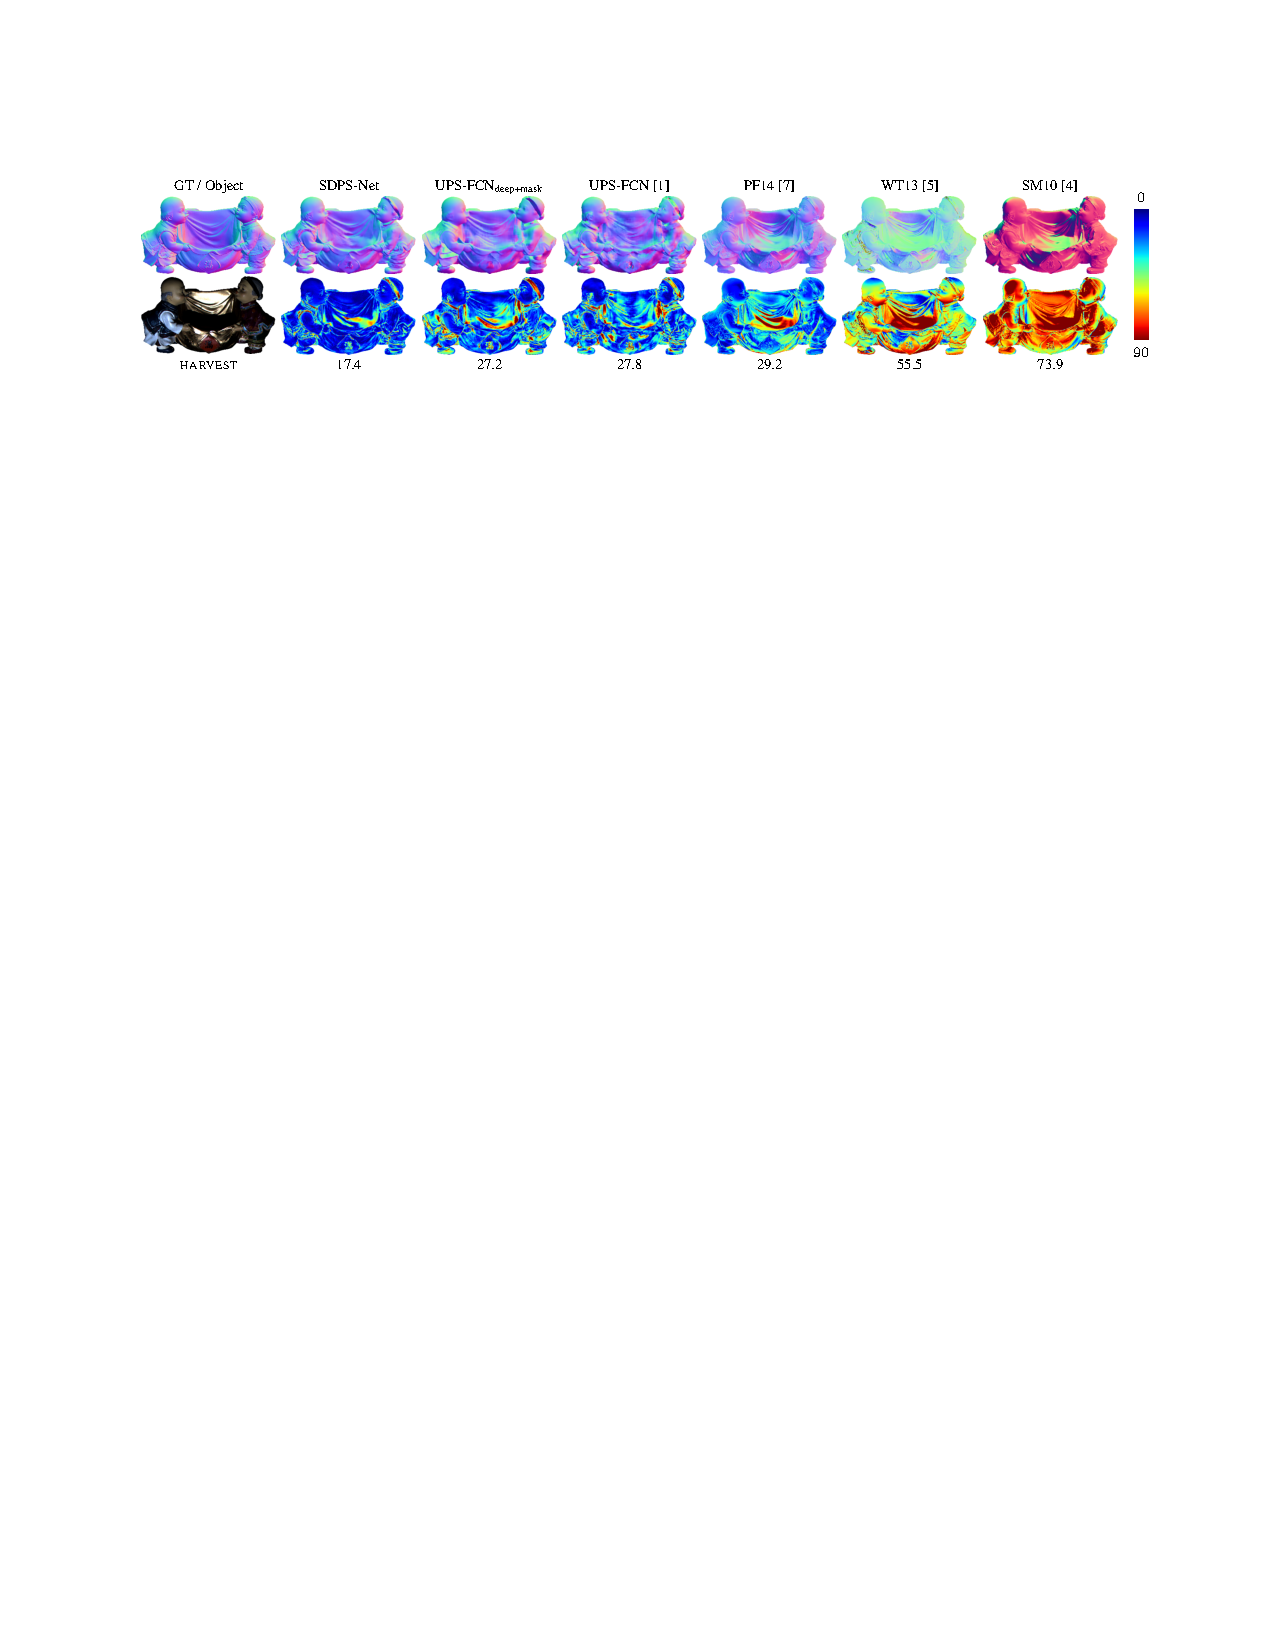
\includegraphics[width=\textwidth]{images/qual_diligent_harvest.pdf}
    \end{center}

    \vspace{-0.8em}
    \begin{minipage}[t]{0.72\textwidth}
        \textbf{\color{blue}Qualitative Results on Gourd\&Apple Dataset~[11] and Light Stage Data Gallery~[12]:} \\
        \vspace{-1.5em}
        \begin{center}
            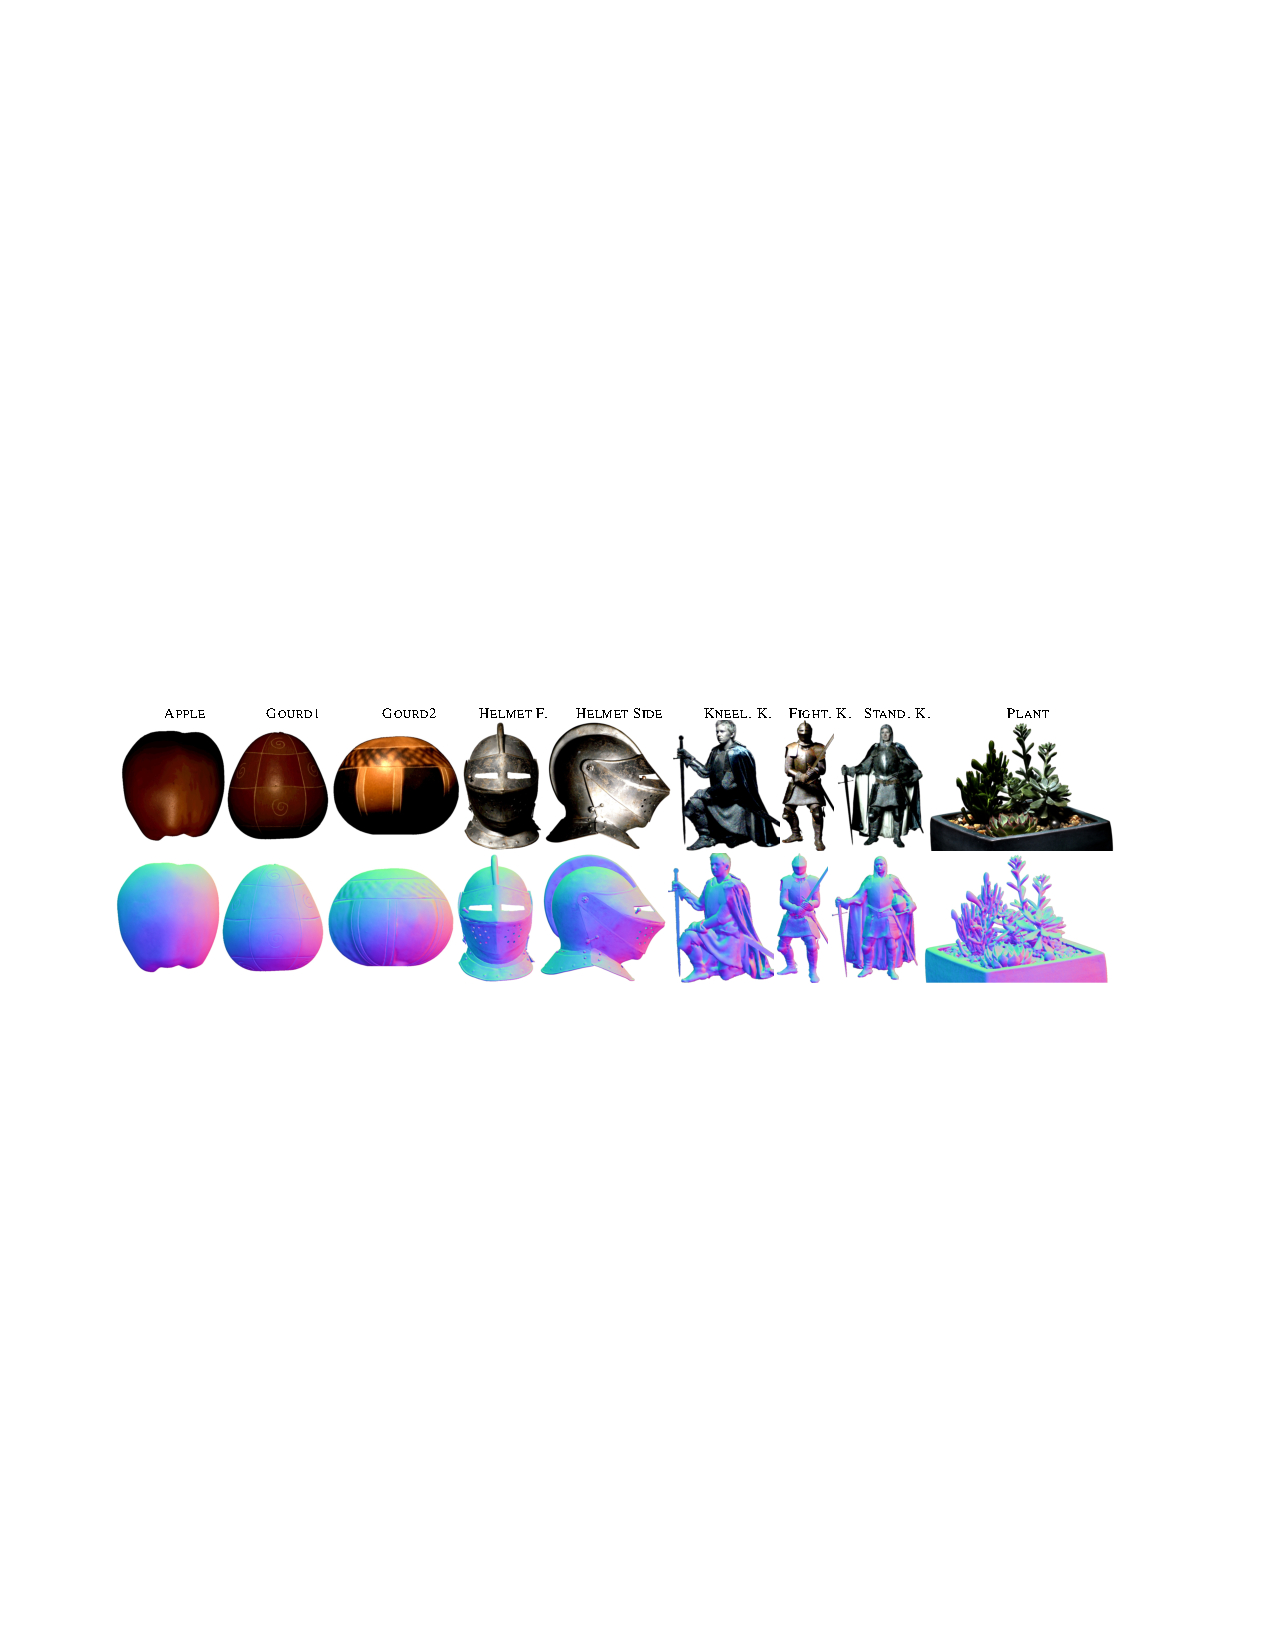
\includegraphics[width=\textwidth]{images/qual_others.pdf}
        \end{center}
    \end{minipage}
    \begin{minipage}[t]{0.28\textwidth}
    \textbf{\color{blue}References:} \\
        \vspace{-1.0em}
        \begin{enumerate}[label={[\arabic*]}]
            \footnotesize
            \item UPS-FCN [Chen~\emph{et al.}, ECCV8]
            \item DiLiGenT [Shi~\emph{et al.}, TPAMI19]
            \item AM07 [Alldrin~\emph{et al.}, ICCV07]
            \item SM10 [Shi~\emph{et al.}, CVPR10]
            \item WT13 [Wu and Tan, CVPR13]
            \item LM13 [Lu~\emph{et al.}, CVPR13]
            \item PF14 [Papadhimitri and Favaro, IJCV14]
            \item LC18 [Lu~\emph{et al.}, TPAMI18]
            \item L2 [Woodham, OE1980]
            \item IS18 [Ikehata, ECCV18]
            \item Gourd\&Apple [Alldrin~\emph{et al.}, CVPR08]
            \item Light Stage [Einarsson~\emph{et al.}, EGSR06]
        \end{enumerate}
    \end{minipage}
}
\end{poster}
\end{document}
